\chapter{JK Flip Flop}
%\ref{sec:background}.

\section{Aim}
%\label{sec:objectives}
To verify Truth Table of JK flip-flop and analyse its circuit with the help of LED's output.

\section{Apparatus}
%\label{sec:objectives}
\begin{itemize}
	\tightlist
	\item Kit for realization of NAND, NOR gates.
	\item Connecting Leads
\end{itemize}

\section{Theory}
	A flip flop is an electronic circuit with two stable states that can be used to store binary data. The stored data can be changed by applying varying inputs. Flip-flops and latches are fundamental building blocks of digital electronics systems used in computers, communications, and many other types of systems.
	
	There are 4 types of flip-flops:
	\begin{enumerate}
		\tightlist
		\item R-S flip flop
		\item D flip flop
		\item J-K flip flop
		\item T flip flop
	\end{enumerate}

	The basic NAND gate RS flip flop circuit is used to store the data and thus provides feedback from both of its outputs again back to its inputs. The SR flip flop actually has three inputs: SET, RESET and clock pulse. In a RS flip-flop the input $R=S=1$ leads to an indeterminate output. The RS flip-flop circuit may be re-joined if both inputs are 1 than also the outputs are complement of each other. This type of flip-flop is known as J-K flip flop

\section{Circuits}
\begin{figure}[ht]
	\centering
	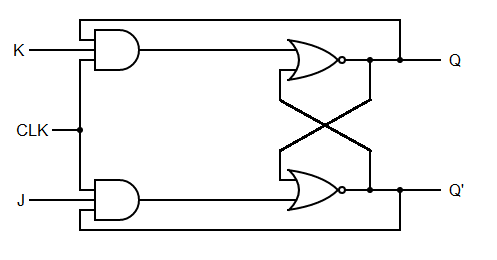
\includegraphics[width=0.6\textwidth,valign=c]{img/exp6/fig1}
	\label{fig:JK_flipflop_circuit}		
	\caption{\textit{JK Flip Flop Circuit Diagram}}
\end{figure}


\section{Procedure}
\begin{enumerate}
	\tightlist
	\item Connect the $1^{st}$ lead to the K terminal of JK flip flop.
	\item Connect the $2^{nd}$ lead to the J terminal of JK flip flop.
	\item Connect clock to CLK terminal of JK flip flop
	\item Connect the $Q$ terminal to one of the output LEDs.
	\item Connect the $\overline{Q}$ terminal to other of the output LEDs.
	\item Turn the power supply on.
	\item Set the input and click on CLK PULSE button.
	\item Observe the output.
	\item Repeat the above three steps for different inputs and note them down.
\end{enumerate}

\section{Observation}
We observe the following values for the Output of JK flip flop:
\begin{figure}
	\centering
			\begin{tabular}{|c|cc|cccc|c|}
				\hline
				\multirow{2}{*}{Trigger} & \multicolumn{2}{c|}{\multirow{2}{*}{Inputs}}                 & \multicolumn{4}{c|}{Output}                                                                                & \multirow{3}{*}{Inference} \\ \cline{4-7}
				& \multicolumn{2}{c|}{}                                        & \multicolumn{2}{c|}{Present State}                             & \multicolumn{2}{c|}{Next State}           &                            \\ \cline{1-7}
				$CLK$                    & \multicolumn{1}{c|}{$J$}                & $K$                & \multicolumn{1}{c|}{$Q$} & \multicolumn{1}{c|}{$\overline{Q}$} & \multicolumn{1}{c|}{$Q$} & $\overline{Q}$ &                            \\ \hline
				$X$                      & \multicolumn{1}{c|}{$X$}                & $X$                & \multicolumn{2}{c|}{-}                                         & \multicolumn{2}{c|}{-}                    & Latched                    \\ \hline
				$\uparrow$               & \multicolumn{1}{c|}{\multirow{2}{*}{0}} & \multirow{2}{*}{0} & \multicolumn{1}{c|}{0}   & \multicolumn{1}{c|}{1}              & \multicolumn{1}{c|}{0}   & 1              & \multirow{2}{*}{No change} \\ \cline{1-1} \cline{4-7}
				$\uparrow$               & \multicolumn{1}{c|}{}                   &                    & \multicolumn{1}{c|}{1}   & \multicolumn{1}{c|}{0}              & \multicolumn{1}{c|}{1}   & 0              &                            \\ \hline
				$\uparrow$               & \multicolumn{1}{c|}{\multirow{2}{*}{0}} & \multirow{2}{*}{1} & \multicolumn{1}{c|}{0}   & \multicolumn{1}{c|}{1}              & \multicolumn{1}{c|}{0}   & 1              & \multirow{2}{*}{Reset}     \\ \cline{1-1} \cline{4-7}
				$\uparrow$               & \multicolumn{1}{c|}{}                   &                    & \multicolumn{1}{c|}{1}   & \multicolumn{1}{c|}{0}              & \multicolumn{1}{c|}{0}   & 1              &                            \\ \hline
				$\uparrow$               & \multicolumn{1}{c|}{\multirow{2}{*}{1}} & \multirow{2}{*}{0} & \multicolumn{1}{c|}{0}   & \multicolumn{1}{c|}{1}              & \multicolumn{1}{c|}{1}   & 0              & \multirow{2}{*}{Set}       \\ \cline{1-1} \cline{4-7}
				$\uparrow$               & \multicolumn{1}{c|}{}                   &                    & \multicolumn{1}{c|}{1}   & \multicolumn{1}{c|}{0}              & \multicolumn{1}{c|}{1}   & 0              &                            \\ \hline
				$\uparrow$               & \multicolumn{1}{c|}{\multirow{2}{*}{1}} & \multirow{2}{*}{1} & \multicolumn{1}{c|}{0}   & \multicolumn{1}{c|}{1}              & \multicolumn{1}{c|}{1}   & 0              & \multirow{2}{*}{Toggles}   \\ \cline{1-1} \cline{4-7}
				$\uparrow$               & \multicolumn{1}{c|}{}                   &                    & \multicolumn{1}{c|}{1}   & \multicolumn{1}{c|}{0}              & \multicolumn{1}{c|}{0}   & 1              &                            \\ \hline
			\end{tabular}
	\label{fig:JK_flipflop_table}		
	\caption{\textit{JK Flip Flop Truth Table}}	
\end{figure}
\section{Precautions}
\begin{enumerate}
	\tightlist
	\item The leads must be connected properly.
	\item Wires must be connected during power supply being off only.
	\item Change the input switches only when supply is off.
\end{enumerate}

\section{Result}
The Truth Table of JK Flip Flop is verified.